\documentclass{article}

\usepackage[utf8]{inputenc}
\usepackage[T1]{fontenc}
\usepackage[french]{babel}

\usepackage{caption}
%\usepackage{pgfplots}
\usepackage{listings}
\usepackage{graphicx}
\usepackage{footnote}
\usepackage{amsmath}
\usepackage{amsthm}
\usepackage{graphicx}
\usepackage{url}
\usepackage{amssymb}
\usepackage{mathrsfs}
\usepackage{multirow}
\usepackage{amsfonts}
\usepackage[boxed,linesnumbered,noend]{algorithm2e}
\usepackage{qcircuit}
\usepackage{enumerate}
\usepackage{eurosym}

\newtheorem{thm}{Theorem}
\newtheorem{prop}{Propriety}
\newtheorem{lemma}{Lemma}
\newtheorem{defi}{Definition}
\newtheorem{coro}{Corollary}

\SetKwBlock{Label}{}{}
\SetKwRepeat{Do}{do}{while}
\SetKwBlock{Void}{void}{}
\SetKwBlock{Struct}{struct}{}

\setlength{\oddsidemargin}{0pt}
% Marge gauche sur pages impaires
\setlength{\evensidemargin}{0pt}
% Marge gauche sur pages paires
\setlength{\textwidth}{470pt}
% Largeur de la zone de texte 
\setlength{\topmargin}{0pt}
% Pas de marge en haut
\setlength{\headheight}{13pt}
% Haut de page
\setlength{\headsep}{10pt}
% Entre le haut de page et le texte
\setlength{\footskip}{40pt}
% Bas de page + séparation
\setlength{\textheight}{630pt}
% Hauteur de la zone de texte

\title{Programmation Avancée des Architecture Multicoeurs}
\author{Gaël Thomas\\
\url{gael.thomas@telecom-sudparis.eu}\\
\url{http://www-inf.telecom-sudparis.eu/COURS/chps/paam/}}
\date{}

\newcommand{\note}{\medskip\noindent\underline}

\begin{document}
\maketitle
\tableofcontents
\newpage


Technique d'optimisation bas niveau (ASM) sur des architectures de "petits multicolores" (environ 30 cœurs). Pas d'OpenMP, pas de MPI (trop haut niveau).

\paragraph{Référence} \emph{The Art of parallel programming}, M.Herlihy, N.Shavit (Bible, à acheter !)

\paragraph{Attention} Les transparents n'ont pas été modifiés depuis 7 ans : ne pas trop s'y fier (50\% d'information données ne sont plus dans les slides en fait).

\section{Introduction}
Depuis une dizaine d'année, les appareils informatiques ont complètement changé (bepuis les tours laides en plastiques...). D'un côté l'informatique embarqué (téléphones, voitures, trains, ...) s'est développée, avec peu de ressources de calcul $\to$ modèle du \emph{mainframe} : serveur/terminaux. Les centres de données sont désormais propulsés par des architectures multicoeurs (le dégagement thermique augmente avec le carré de la fréquence, on augmente donc le nombre de coeurs car l'augmentation est linéaire avec la consommation). La loi de Moore restant toujours possible (miniaturisation des transistors), on intègre des clusters de machine complet sur un die.

De nos jours, pour gagner des performances, il faut augmenter le parallélisme, ce qui est difficile. Nous allons bien entendu travailler dessus, ainsi que sur le placement (caches).

On a un aspect de plus en plus nomade de l'informatique (on masque la localisation : possibilité de continuer un travail sur plusieurs machine), rendu possible par la centralisation des calcul. La technique utilisée est la \emph{virtualisation}, ce qui est également possible pour le HPC. On n'utilise quasiment plus la machine telle qu'elle est. L'idée est d'utiliser une "machine dans une machine", ce qui introduit une \emph{couche de virtualisation} qui modifie les comportement\footnote{il s'agit du sujet de recherche de notre professeur}.

\paragraph{Plan}
\begin{enumerate}[I]
\item Etude des multicoeurs (NUMA) $\to$ TP très sympa pour mesurer la latence mémoire
\item Concurrence en mémoire partagée
\item Algorithme classique et sans verrous
\item Mémoire transactionnelle
\end{enumerate}


\subsubsection*{Rappel sur les verrous (mutex)}
Les threads lisent et écrivent des valeurs dans un \emph{registre} en mémoire, par exemple une base de donnée d'une banque lue et écrit par des distributeurs. Certains registres sont en lecture, lecture/écriture, écriture. On s'intéresse ici aux registres en lecture/écriture.

Le problème réside dans le fait qu'il est possile d'avoir des accès \emph{concurrents} qui mènent à des données \emph{incohérentes} (du point de vue du programmeur !). C'est le problème du \emph{chat-mouton} (essayer de dessiner un chat et un mouton sur le même tableau par deux enfants, ça ne va pas trop marcher...).

\paragraph{Problème classique des bases de données sur lequel est basé tout le cours :} Les comptes en banque. Un processus $p_1$ lit le compte et le met à jour en ajoutant deux euros. Un ami, processus $p_2$ est avec votre carte bleue et débite 100\euro (lire le compte puis le met à jour). Il est possible de miraculeusement gagner 100\euro : 
\begin{itemize}
\item[$p_1$ :] $a$ lit le contenu ($cpt=100$\euro)
\item[$p_1$ :] ajoute 2 à $a$ ($cpt=100$\euro, $a=102$\euro)
\item[$p_2$ :] $b$ lit le compte ($cpt=100$\euro)
\item[$p_2$ :] retirer 100 à $b$ ($cpt=100$\euro)
\item[$p_2$ :] $b$ devient le nouveau solde ($cpt=0$\euro)
\item[$p_1$ :] $a$ devient le nouveau solde ($cpt=102$\euro)
\end{itemize}
\bigskip

Le retrait a disparu ! Pour palier à ce fait, on utilise un verrou pour retirer l'accès concurrent. Les régions dangereuses sont appelées \emph{sections critiques} et doivent être exécutés \emph{atomiquement}. Le verrou joue le rôle de feu de signalisation pour les programmes : tant que le verrou n'est pas libre j'attends, si il est là je le prends et je suis le seul à pouvoir le prendre.

On entoure les section critiques par le verrou:
\begin{algorithm}
lock(mutex) \tcp*{bloquant si jamais le mutex n'est pas disponible}
\tcc{section critique 1\;
Par exemple ajouter 2\euro\;}
unlock(mutex)\;
\end{algorithm}

\begin{algorithm}
lock(mutex) \tcp*{bloquant si jamais le mutex n'est pas disponible}
\tcc{section critique 2\;
Par exemple retirer 100\euro\;}
unlock(mutex)\;
\end{algorithm}

\paragraph{Attention aux situations de famines !} Il ne faut pas qu'une suite d'opérations menant à un interbloquage des threads soit possible ! Il faut éviter d'inverser l'ordre des verrous (dans la doc Linux par exemple, il est indiqué dans quel sens prendre les verrous !).


\paragraph{Petit aparté} Attention, cela revient rapidement costaud niveau math derrière, le parti pris ici est de retirer le maximum de la théorie pour passer au code.

\paragraph{Notation} Un exam final sur 100\% et un devoir surprise à un moment sur 10\%. Une annale sont disponibles sur le site (attention, ne pas se fier à la difficulté car elle dépend de la promo).

\paragraph{Conseil} Garder un œil sur les revues scientifique, même si vous vous destinez à un parcours d'ingénieur (grrrr...\footnote{Humour : L'auteur de ces notes ne se destine pas à ce parcours, ne vous vexez pas}).


\section{Architectures des Machines Multicoeurs}
Idée : comprendre au niveau matériel et pourquoi certains comportement au niveau logiciel peuvent sembler étranges.

\emph{Auparavant} Loi de Moore : la densité d'intégration des transistors double tout les 18 mois. Cette puissance permettait d'augmenter la fréquence, qui s'est heurtée à la dissipation thermique (la consommation augmente avec le carré de la fréquence). On sait par contre que ça ne sera pas toujours le cas : les interconnexions entre coeurs peuvent également tirer beaucoup d'énergie, bien que ce ne soit pas le facteur limitant de nos jours.

De nos jours, il est possible de louer des serveurs vers 80 cœurs par Amazon : c'est le \emph{cloud computing}.
\bigskip

\paragraph{Premier grand problème:}
Il faut paralléliser le code ! Et ce n'est pas suffisant.
\bigskip

Au niveau architecturale, il est impossible d'utiliser une topologie classique à base de bus, car environ une instruction sur quatre est un accès mémoire. Pour palier à cela, on change la topologie : \emph{diviser pour mieux régner}. On utilise un bus pour relier plusieurs cœurs entre eux et former une \emph{nœuds} de calcul, puis on les relies entre eux.
\bigskip

\paragraph{Terminologie}
\begin{itemize}
\item[Unité de calcul :] capable de faire des additions/opération (on appelait cela processeur auparavant
\item[Unité mémoire :] Contrôleur permettant la traduction adressage virtuelle/physique
\item[Contrôleur d'interruption :] Gère les interruptions (principalement par les périphériques
\item[Un timer :] Indépendant par cœur (imaginez si une seule horloge à 800 kHz devait communiquer chaque tick au 50 cœurs...). Lors de l'utilisation de l'instruction \texttt{rtsc} (read timestamp counter), ceux-ci sont légèrement différents entre cœurs.
\item[Un cache (donnée et code)]
\item[Le TLB (translation lookout buffer) :] Stocke les mapping mémoire virtuelle/physique récents
\end{itemize}

L'ensemble de ces éléments est appelé un \emph{tuile} ou \emph{cluster} qui sont intégrés sur des \emph{die}. Ce dernier correspond à un circuit intégré unique (souvent, il s'agit d'un cluster). Une \emph{socket} est l'objet physiquement déplaçable contenant un ou plusieurs dies. Attention, cela n'est pas lié au NUMA, qui est lui une construction logicielle (bien que proche).

Le \emph{Network On Chip} est la partie qui connecte les différent coeurs d'un die. Ce qui connecte les dies ensemble est appelé \emph{Inter-connect}.

\begin{figure}[h]
\centering
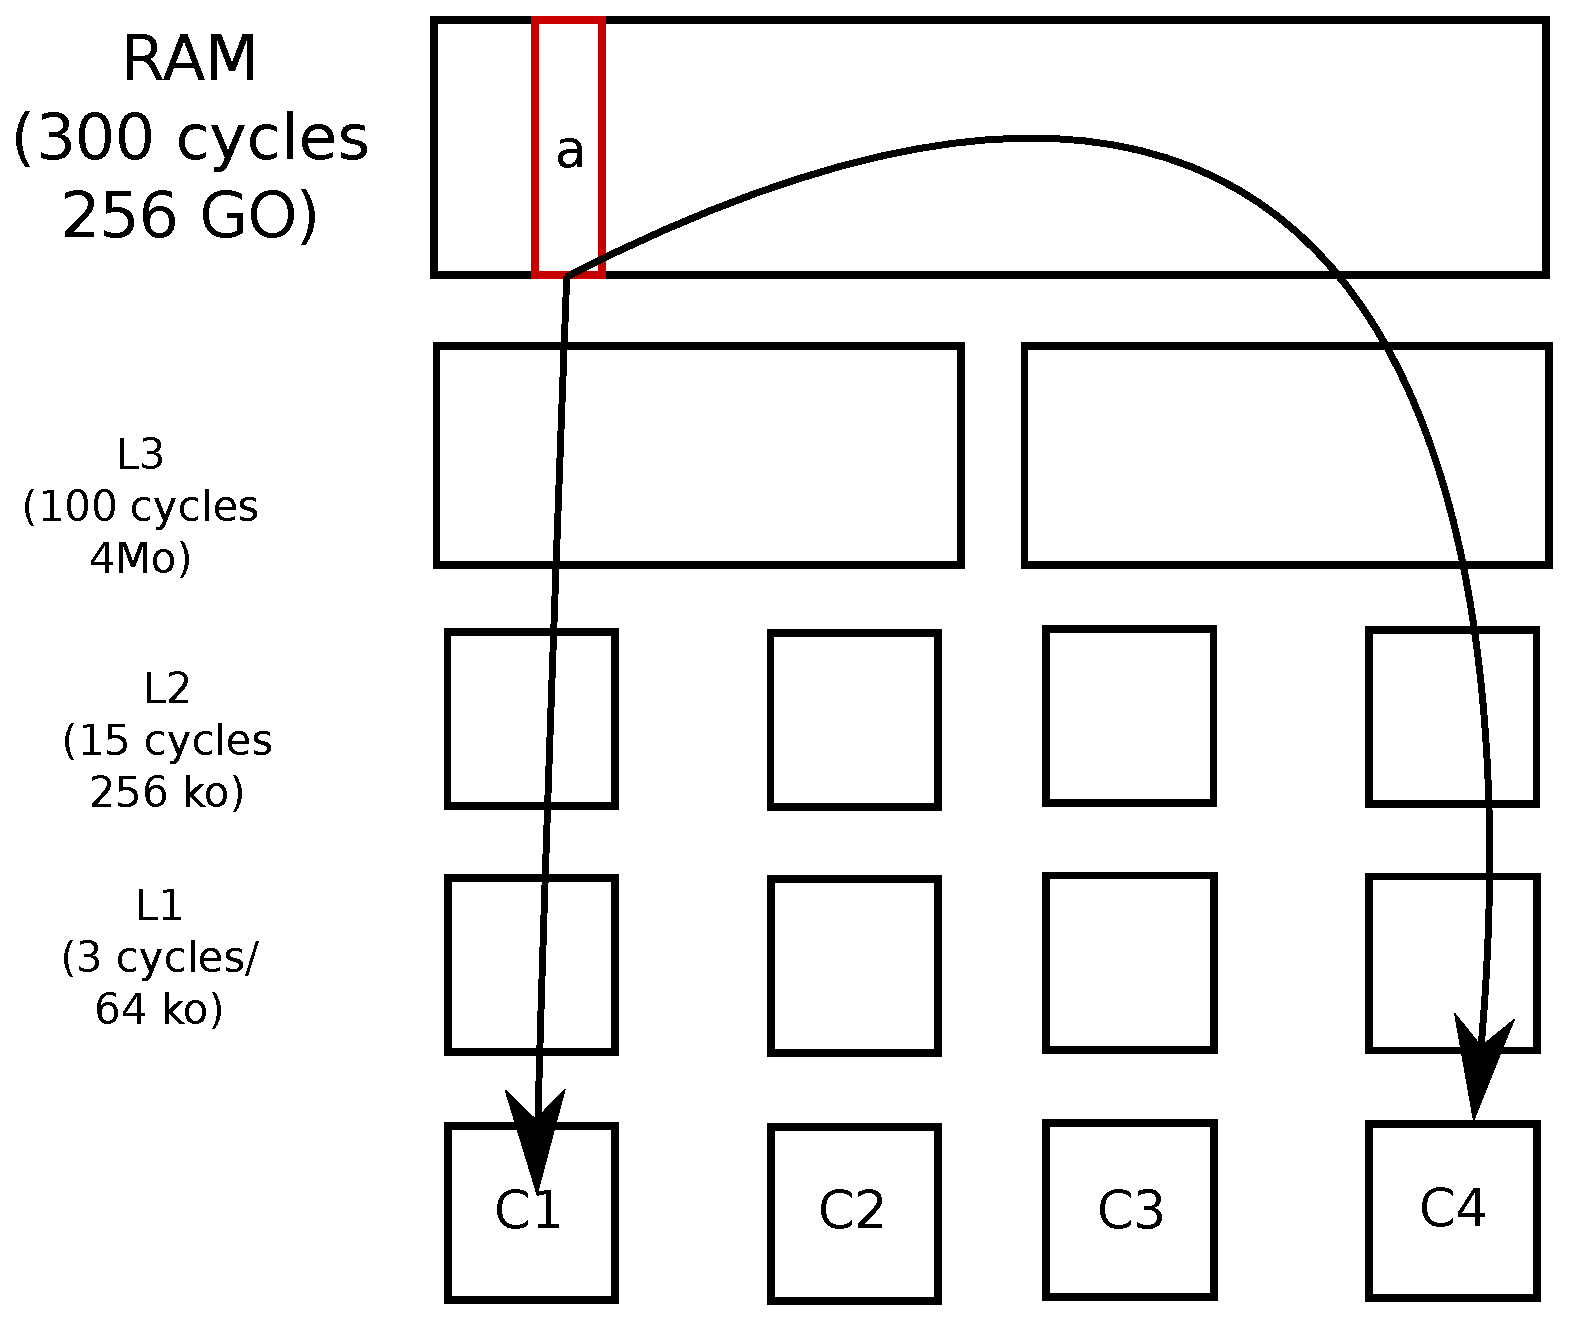
\includegraphics[width=0.5\linewidth]{cache.eps}
\caption{\label{fig:cache}Hiérarchie des caches}
\end{figure}

\subsection{Problème du cache}
Il assure la cohérence des données, donne un sens à ce que le processeur voit de la mémoire (cf figure \ref{fig:cache}). Comment invalider une ligne de cache en cas de modification ?

On utilise le processus MOESI : un verrou contenant un état par ligne de cache\footnote{c'est ce problème qui est à l'origine du NUMA}, la synchronisation s'effectuant entre cache de même hiérarchie :
\begin{itemize}
\item[E :] Excusive (Écriture)
\item[I :] Invalid (A été modifiée / plus présente)
\item[S :] Shared (Lecture)
\end{itemize}
Il faut cependant garder l'information "la valeur en cache est-elle plus récente que celle en RAM ?". Pour cela, on dédouble tous les états :
\begin{itemize}
\item[M :] Modified, E mais incohérente avec la mémoire centrale
\item[O :] Owned, S mais incohérente avec la mémoire centrale
\end{itemize}
L'état I n'est pas répliqué puisque la ligne de cache n'a plus aucun sens.
\bigskip

Pour récapituler :
\begin{itemize}
\item[État M ou E :] verrou en écriture
\item[État O ou S :] verrou en lecture
\item[État I :] pas de verrou
\end{itemize}
\bigskip

Où est le soucis ? Avant, on faisait du \emph{snooping} (espionnage) : tout passait par le bus. Le soucis est que le snooping ne scale pas car il demande un \emph{broadcast} (demander à toutes les autres cœurs).

Solution : On segmente la mémoire en centralisant l'accès à certaines lignes de caches qui sont gérés par certains clusters spécifiques. Des tables associent les adresses physiques aux cœurs qui cachent la ligne : ainsi les invalidation seront spécifiquement envoyés au bon processeur. Autre soucis : où mettre la table ? La segmentation se fait en divisant la mémoire par le nombre de cluster et en répartissant équitablement celle ci entre les cluster (noeud 1 $\to$ mémoire de 0 à 2 Go, noeud 2 $\to$ 2 à 4 Go, etc). Le cluster est alors un \emph{nœud NUMA}, qui correspond souvent à un die (bien que ce soit trois dénominations différentes). Le routage s'effectue par chaque nœud NUMA qui connait la table (stockée dans le L3 et gérée par un petit contrôleur), spécifiée pas le BIOS au démarrage.

\paragraph{Note :}
Cette segmentation est nécessaire mais relativement peu utilisée (bcp de variables locales). Dans le meilleur des cas (pas de saturation), une lecture va couter environ 500 cycle. Dans le cas saturé, environ 2000 cycles !

\paragraph{Conséquences :}
L'accès à la mémoire centrale n'est plus uniforme (local : 200 cycles ; au pire, 400 cycles) ; les liens peuvent saturer (et là, 2000 cycles !). La partitionnement de la mémoire change la latence !

\paragraph{Principe/Solution :} augmenter au maximum la localité quand on développe une appli. Par défaut, la mémoire virtuelle est mappée sur différents nœuds NUMA selon la politique \emph{first touch} : si la mémoire n'est pas encore mappée, on lui donne de la mémoire à partir \emph{de son propre noeud}. Dans le cas de gros malloc, le mappage se fait \emph{au niveau des premiers accès} et non au niveau de la réservation.

Il existe également l'\emph{interleaved} qui utilise un \emph{round robin} (allocation aléatoirement de la mémoire), ce qui permet d'équilibrer les accès mais est très mauvais pour la localité (pas de saturation interne).

\subsection{Placement de processus sous Linux}
\texttt{pthread\_setaffinity} pour sélectionner le cœur, \texttt{mbind} pour n'allouer la mémoire physique qu'à partir d'un ensemble de nœuds. \texttt{madvise} permet de libérer les pages physiques pour les migrer. Pour plus de détails, voir le manuel linux (\texttt{man fonction}).


\section{Algorithmique sans verrou}
Le principe même du verrou induit des threads inactifs lorsque ce dernier est pris (verouillé). En fait, plus il y a de verrous, moins il y a de parallélisme ! Le verrou force la séquencialisation de la section critique.

Le principe des \emph{structures non bloquantes} est née dans les années 80, puis a connu un nouvel essor en 200 avec la liste chainée sans verrou. 
\bigskip

\begin{defi}[Loi d'Ambdahl]
Pour tout programme, si $p$ est la proportion de code exécutable en parallèle, $\dfrac{p}{n}$ la répartition de la charge de travaille sur $n$ cœurs, alors l'accélération maximal théorique est 
\[a = \dfrac{1}{1 - p + \dfrac{p}{n}} \;\underset{n\to +\infty}{\longrightarrow}\; \dfrac{1}{1-p}\]
\end{defi}

Cela signifie par exemple que pour une un programme parallélisé à 75\%, l'accélération maximale sera de 4 (3,7 à 32 cœurs). Pour un taux de parallélisation de 95\%, le speedup maximal est de 20, et atteint 100 pour un code à 99\% parallélisé.

\paragraph{Note}
La formule donne également une idée du nombre de cœurs "utiles". Par exemple, pour un code à 95\% parallèle, le speedup passe de 12,55 à 32 cœurs à 17,42 à 128 cœurs).

\paragraph{Conclusion} Cela vaut le coup de se battre \emph{pour quelques pourcents de parallélisation}, même pour une addition seule !

\paragraph{Exemple}
\begin{itemize}
\item Une addition (\texttt{x++}) sur la suite SPARC 2) permet de multiplier les performances par 10 sur 50 cœurs !
\item Le compteur d'ouverture des fichiers était le goulot d'étranglement de Linux sur le HPC (meilleur papier système 2013)
\end{itemize}

\paragraph{Comment se passer du code séquentiel ?}
Retirer la mémoire centrale. C'est cependant impossible, même sur MPI, les \texttt{gather}/\texttt{scatter} cachent une synchronisation dans la répartition des résultats.


Dans les grands centres web par exemple, tout est fait avec des processus (communication par TCP/IP au lieu de la mémoire partagée).

\subsection{Solution naturelle}
Qu'est-ce qu'un algorithm non bloquant ?

\begin{itemize}
\item[Wait-free :] Toute opération se termine en un nombre fini de pas (i.e. pas de blocage de threads ni de famine). Cela est peu utile en HPC car il contient beaucoup de code séquentiel (et donc non parallélisable) ; mais est très recherché dans le domaine du temps réel.
\item[Lock-free :] Si des opérations sont appelée infiniment souvent, alors elles se terminent infiniment souvent (ceci est une garantie \emph{asymptotique} donc pas de garantie temporelle, pas de bornes). $\to$ pas d'interblocage du programme, mais certains threads peuvent ne jamais être élus).
\item[Obstruction-free :] A tout moment, tout thread s'exécutant seul termine son opération en un nombre fini de pas (i.e. pour tout temps $t$ je peux couper tous les threads sauf un et terminer l'exécution de ce threads en un temps fini).
\end{itemize}
\bigskip

Noter que
\[\text{Wait-free} \Rightarrow \text{Lock-free} \Rightarrow \text{Obstruction-free}\]
Les algorithmes à verrou ne sont pas obstrution-free, car une fois le verrou pris, tous les autres threads sont bloqués.
\bigskip

Du point de vue des adversaires :
\begin{itemize}
\item[Wait-free :] On borne le temps maximal perdu par l'adversaire
\item[Lock-free :] L'adversaire peut retarder de manière arbitrairement grande mais pas infiniment souvent
\item[Obstruction-free :] Pas d'adversaire vu que l'on coupe les autres threads
\end{itemize}

\subsection{Structures non bloquantes}
\subsubsection{Les outils}
On redescend au niveau architectural : les outils sont fournis par le processeur :
\begin{itemize}
\item \texttt{old-value $\leftarrow$ atomic-add(variable, value)} \emph{sans verrou} (il s'agit d'un verrou sur une ligne mémoire pendant le temps de l'opération $\to$ temps d'exécution borné)
\item \texttt{old-value $\leftarrow$ atomic-swap(variable, value)} écrit un valeur en mémoire et renvoie son ancienne valeur
\item \texttt{old-value $\leftarrow$ atomic-CAS(variable, test, new)} : atomic compare and swap : compare et échange la variable si et seulement si elle vaut \texttt{test}. Dans tous les cas, la valeur initiale de la variable est retournée.
\end{itemize}

D'un point de vu théorique, $atomic-CAS$ à la puissance du consensus (si on vote sur la valeur, à la fin tout le monde à voté sur une valeur proposé et tout le monde est au courant du résultat). Sur le plan logique pure, \texttt{atomic-add} et \texttt{atomic-CAS} sont équivalents, \texttt{atomic-swap} est plus faible.

\paragraph{Exemple} \texttt{add} atomic en obstruction-free en utilisant \texttt{atomic-CAS}:\\
\begin{algorithm}[H]
\Void({add (int* x, int a)}){
	int old, new\;
	\Do{atomic-CAS(x, old, new)}{
	old = *x\;
	new = old + a\;
	}
}
\end{algorithm}
\bigskip

Locking mechanism in Linux: ticket-lock\\
\begin{algorithm}[H]
int ticket\;
int billet\;
\Void({lock()}){
	int billet = atomic-add(\&ticket,1)\;
	\While{guichet$<$billet}{
		wait()\;
	}
}

\Void({unlock()}){
	atomic-add(\&guichet,1)\;
}
\end{algorithm}

Noter que \texttt{atomic-CAS} est un lock en lui-même, appelé \texttt{spinlock}.
\begin{algorithm}
\Void({lock()}){
	\While{CAS(\&l, 0, 1) == 1}{
		wait()\;
	}
}
\Void({unlock()}){
	l=0\;
}
\end{algorithm}
\paragraph{Attention} Ne JAMAIS l'utiliser : l'attente est \emph{active} (besoin de lecture \emph{et écriture}), ce qui sature le bus !


\subsubsection{Modèles mémoire}
Il définit les ordonnancements possibles des accès mémoires. Un exemple de problème :

\begin{algorithm}[H]
\Label(send){
	msg = "coucou"\;
	recu = true\;
}

\Label(recv){
	\While{recu==false}{
		printf(msg)\;	
	}
}
\end{algorithm}
A cause des écriture différés du processeur, il est pourrait être possible que la valeur lue par \texttt{printf} ne soient pas encore écrite en mémoire.
\bigskip

Chaque processeur donne des garanties spécifiques. Un principe commun est qu'en local ($\Rightarrow$ pour le même thread), toute lecture succédant à un écriture lit la dernière valeur écrite.

\begin{figure}[h]
\centering
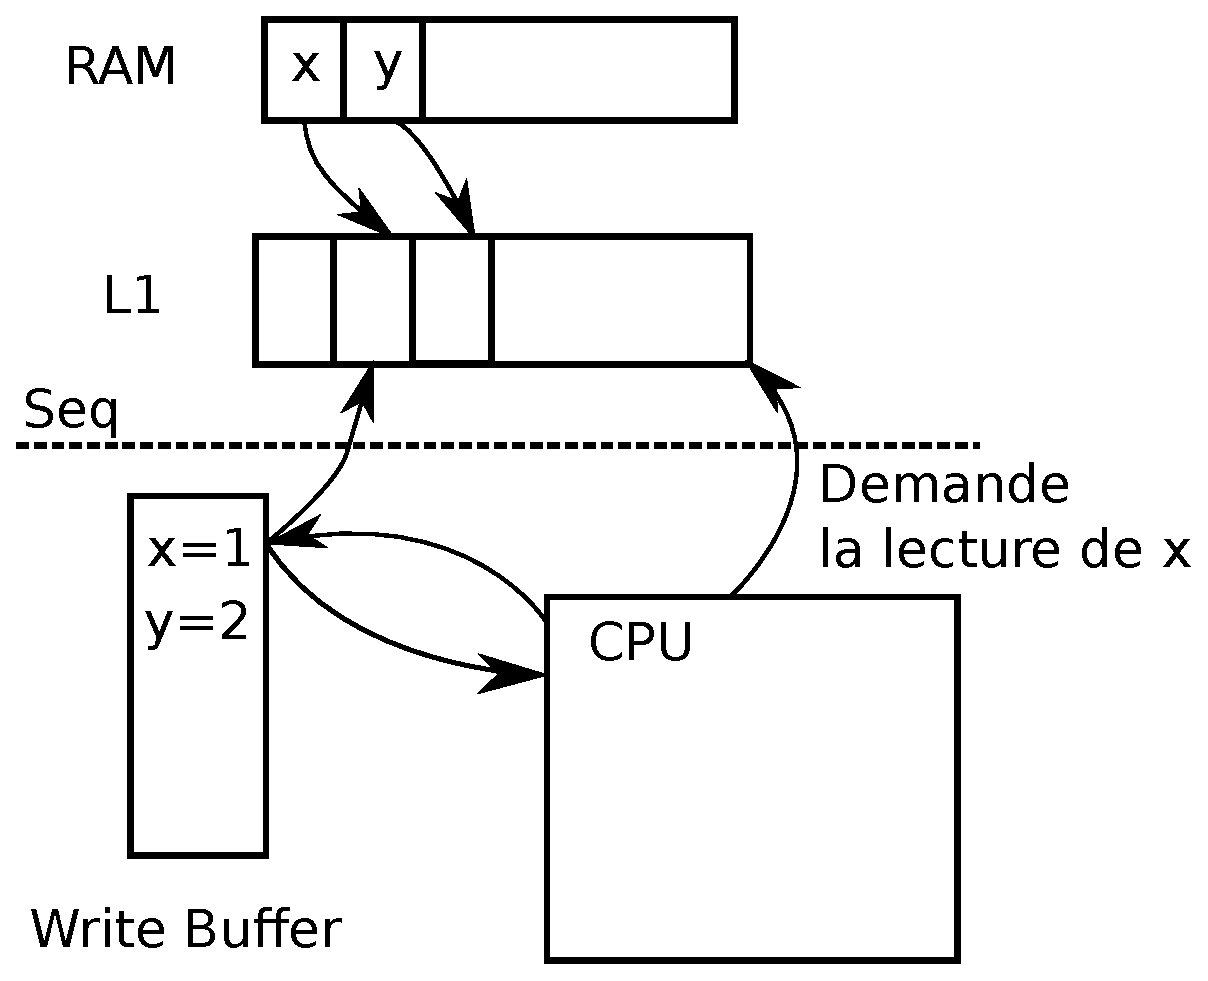
\includegraphics[width=0.5\linewidth]{write_buffer.eps}
\caption{\label{fig:write_buffer}Principe du Write Buffer}
\end{figure}

De manière similaire, il existe également un Read Buffer de principe similaire au Write Buffer (mais implémenté à des endroit différents).

\paragraph{Information} Chaque écriture du cache est précédé d'une lecture, car le cache est accessible ligne par ligne, il faut donc conserver les anciennes données.
\bigskip

Le modèle du X86 est le \emph{TSO : Total Store Order}
\begin{itemize}
\item Les lectures ne sont jamais réordonnancées entre elles
\item Les écritures non plus
\item Une écriture après une lecture n'est pas réordonnancée
\item Une lecture après un écriture peut être réordonnancée s'il s'agit de deux cases mémoires distinctes
\end{itemize}
\bigskip

Si jamais un des ces cas devait arriver, le buffer responsable de la seconde opération consulte l'autre buffer, et on attend que la première opération soit propagée en mémoire (ce qui est un trou à performances, mais nécessaire pour la programmation.

\paragraph{Attention à la lecture après écriture dans deux cases mémoires distinctes} Bien que en pratique ça ne soit pas dérangeant.
Initialement : $t_1=t_2=0$.
\begin{itemize}
\item[$P_1$ :]écrit $x$, 2\\
$t_1=$ lit $y$
\item[$P_2$ :]écrit $y$, 1\\
écrit $x$, 1
\item[$P_3$ :]$t_2$ = lit $x$
\end{itemize}
En cohérence séquentielle (sans réordonnancement), il est impossible d'avoir ${x,t_1,t_2}={2,0,1}$. En effet $x=2$ s'effectue avant $x=1$, et la lecture de $x$ s'effectue entre ces deux opérations. Or cela est possible en TSO (la lecture de $t_1$ peut être effectuée en tout premier lieu).

 
Les instructions autorisées sont \texttt{lock xadd}, \texttt{xchg} et \texttt{lock xchg}.

Pour éviter le seul réordonnancement possible, \texttt{mfence} permet une barrière mémoire, qui vide les buffers lecure et écriture. \emph{Attention}, en C, il faut donc en mettre car on ne connait pas la plateforme d'exécution. Le préfixe d'instruction \texttt{lock} intègre automatiquement un \texttt{mfence} ainsi que la visibilité immédiate de l'écriture après l'instruction préfixée.
\bigskip


Il n'y a pas de garantie de réordonnancement en C avant le C11. Cependant il existe des instruction atomique pour les compilateurs, tels \texttt{\_\_sync\_fetch\_and\_add}, \texttt{\_\_sync\_lock\_test\_and\_set} (pour \texttt{xchg}, vraiment bizarre) \texttt{\_\_sync\_val\_compare\_and\_swap}, et la barrière mémoire \texttt{\_\_sync\_synchronisze}. Sur du X86, pas de soucis, mais attention si le code doit être exécuté sur des archi spécifiques. Il en existe un pour C11 ou C++11, mais très relâché.
\bigskip


En Java, tout réordonnancement est possible, mais les variables déclarées \emph{volatiles} génèrent une barrière mémoire à chaque accès. De plus, des barrières seront présentes lors de l'entrée et la sortie des sections critiques.
\bigskip

En particulier, il faut éviter d'utiliser un lock non volatile pour initialiser une variable.

\section{Structures de données}
\subsection{La pile}
Structure \emph{LIFO} : Last In First Out. La pile possède deux méthodes : \texttt{push} (empiler) et \texttt{pull} (dépiler).

\paragraph{Avec des locks :} On verrouille lors des \texttt{push}/\texttt{pop}.

\paragraph{Sans lock :} L'idée est de faire un \texttt{atomic-CAS} sur le pointeur de tête.

\begin{algorithm}[H]
\Void({push(head, element)}){
	\Do{\texttt{atomic-CAS(\&head, n.next, n) != n.next}}{
		Node n = new Node (head, element)\;
	}
	\tcp{Si la tête n'as pas changé, on insère en changeant la valeur de la tête}
}
\end{algorithm}

On voit ici un \emph{point de linéarisabilité} : on ramène \texttt{push} à une seul opération atomique.

Le principe est la même pour \texttt{pop}


\begin{algorithm}[H]
\Void({pop(head)}){
	\Do{\texttt{atomic-CAS(\&head, n, n.next) != n}}{
		Node n = head\;
	}
}
\end{algorithm}

Au niveaux des garanties : \texttt{push} et \texttt{pop} sont obstruction-free (en coupant tous les autres threads, au pire on recommence un seule fois car la tête n'est plus modifiée. Elles sont également lock-free, (se prouve par induction sur le nombre de threads) : si on demande un infinité de push, une infinité est bien exécutée mais pas forcément par tous les threads. Il peut par contre y avoir famine (un thread peut être infiniment bloqué). Par contre, il n'est pas wait-free.


\subsection{La queue}
Il s'agit d'une structure \emph{FIFO} : first in first out. Deux fonctions sont possibles : \texttt{enqueue(element e)} pour ajouter un élément à la tête, et \texttt{dequeue()} pour le retirer. Il y a donc deux pointeurs : \texttt{head} et \texttt{tail} (pointeur de début pour dequeue de fin pour l'ajout de nouveaux élément). Il faut faire attention au cas de liste vide, où l'on doit changer à la fois \texttt{head} et \texttt{tail}.

Pour gérer ces cas embêtants, on rajout un faux noeud (la list ne peut plus être vide). Pour le \texttt{dequeue()} (côté tail), on va utiliser le même algorithme que \texttt{pop()}. On va conserver à tout instant trois invariants :
\begin{itemize}
\item Le premier noeud est en seconde position (la première est le faux noeud)
\item Les listes commençant par \texttt{head} et \texttt{tail} se rejoignent
\item Le dernier noeud est toujours le noeud de queue
\end{itemize}

\begin{algorithm}[H]
\Void({enqueue(Element e)}){
	Node node = new Node (null, e)\;
	\Do{CAS(\&old.next, null, node) != node}{
		Node old = tail\;
		\While{old.next != null}{
			CAS(\&tail, old, old.next)\;
			old = tail\;		
		}	
	}
	CAS(\&tail, old, node)\;
}
\end{algorithm}

Le \texttt{dequeue} est le même qu'avant à l'exception près du faux noeud à ne pas prendre en compte. Dans ce cas, le fake évolue pour être l'élément retiré.




\subsection{La liste chainée}
On va autoriser des noeuds non valides à exister dans la liste : on les marques gris et on les ignore. Pour les griser, on va mettre à 1 le bit de poids faible de pointeur (ce qui ne l'invalide pas car les adresses mémoires sont alignées). Pour accéder au pointeur, on effectue $ptr \; \& \; -2$, pour accéder à la couleur, $ptr \; \& \; 1$.

Les invariants seront alors :
\begin{itemize}
\item La liste est toujours connectée et ordonnée
\item Certains noeuds supprimées peuvent rester dans la liste
\end{itemize}

\begin{algorithm}[H]
\Void({del(coloredPointer* plist, int value)}){
	\Label(restart :){
		coloredPointer* pred = plist\;
		
		
		\While{!found}{
			Node curr = pointer(*pred)\;
			
			\If{curr == null $||$ value < curr$\to$value}{
				\tcp{pas trouvé}
				return\;
			}			
			
			
		
			\If{curr $\to$ value == value}{
				\tcp{trouvé}
				\Do{CAS(\&cur$\to$next, n, n $|$ 1) != n}{
					n = curr $\to$ next\;
				}
			}		
		
		
			\If{mark(curr$\to$mext)}{
				\tcc{curr doit être supprimé}
				\eIf{CAS(pred, curr, pointer(curr$\to$next)) != cur}{
					goto restart\;
					\tcp{On est allé trop loin dans la liste}
				}{
					continue\;
				}
			}				
			
			
			
			pred = \&curr$\to$next\;
		}
	}
}

\end{algorithm}


Ajout :



\begin{algorithm}[H]
\Void({add(coloredPointer* plist, int value)}){
	\Label(restart :){
		coloredPointer* pred = plist\;
		
		
		\While{!found}{
			Node curr = pointer(*pred)\;
			
			 \If{curr == null $||$ value < curr $\to$ value}{
			 	\eIf{CAS(pred, curr, new Node(curr, value)) != curr}{
			 		goto restart\;
			 	}{
					return\;			 	
			 	}
			 }
		
		
			\If{mark(curr$\to$mext)}{
				\tcc{curr doit être supprimé}
				\eIf{CAS(pred, curr, pointer(curr$\to$next)) != cur}{
					goto restart\;
					\tcp{On est allé trop loin dans la liste}
				}{
					continue\;
				}
			}				
			
			
			
			pred = \&curr$\to$next\;
		}
	}
}

\end{algorithm}


L'algorithme est obstruction-free et lock-free mais pas wait-free.

\subsubsection*{Implémentation}
\begin{algorithm}[H]
\Struct(node){
	struct node* next\;
	int value\;
}
\Struct(colorPtr){
	uintptr\_t ptr:63\tcp{indique que l'on prends 63 bit}
	uintptr\_t color:1\;
}
\end{algorithm}
On se force à utiliser des structures sur 64 bits car le CAS utilise des structures 64 bits.
\bigskip

Pour l'implémentation, procéder par étape : d'abord le parcours, puis chaque cas un à un.



\section{Mémoire Transactionnelle}
\subsection{Pourquoi ?}
Les algorithmes lock-free sont très difficiles à implémenter car théoriquement très difficile. Une solution intermédiaire consiste à dégrader quelque peu les performances (souvent plus rapide que le lock, mais légèrement plus lent que le lock-free), mais gagner une simplicité de programmation énorme.

\paragraph{Rappel :} selon la loi d'Amdahl, le facteur prédominant est (en HPC) les quelques pourcents de code non parallélisable. Pour réduire au maximum la séquentialisation, on peut :
\begin{itemize}
\item Utiliser des lock plus nombreux (verrou à grain fin)
\item Utiliser des compare-and-swap
\end{itemize}
Statistiquement, la probabilité de conflit est assez faible, on va donc essayer de supprimer les verrous.
En effet, les verrous fins sont :
\begin{itemize}
\item Difficile à maintenir (\emph{très très important en HPC})
\item Difficilement débogable
\item Difficilement prouvable
\item Difficile à composer (quasi impossible)
\item Effet de bord important : protocole d'accès à une variable implicite (pour accéder à telle variable je dois faire telle chose avant
\end{itemize}

En outre, le verrouillage fin reste très pessimiste. L'idée des mémoires transactionnelles est de faire du verrouillage optimiste. On veut garder \emph{l'atomicité} des sections critiques ($\to$ pas d'intermédiaires vu par les autres threads). On va donc laisser les threads s'exécuter en parallèles, mais revenir à un état antérieur en cas de problème.

On s'attend alors à :
\begin{itemize}
\item simplifier le code : pas besoin de connaître l'ordre des verrous
\item non-deadlock, non-famine, composabilité assurée par la plate-forme
\item on ne bloque un coeur que si c'est nécessaire (i.e. car conflit)
\end{itemize}

Dans la pratique, cela est faux. Parfois on gagne, parfois on perd par rapport à un verrouillage à grain fin, mais on reste plus performant qu'un unique verrou (et moins qu'un lock-free).

\begin{defi}[Bloc atomique]
Un bloc atomique est exécuté de façon atomique. Cela signifie qu'il semble s'exécuter instantanément aux yeux des autres threads.
\end{defi}

Dans ce cas, la programmation devient bien plus simple ; la composition de block atomique est bien plus simple. Le mot-clef \texttt{retry} permet de mettre le thread en attente et de retenter la section transactionnelle lorsqu'une des variables lue avant le retry est modifiée. On peut alors utiliser \texttt{orElse} qui permet d'exécuter une autre section en cas d'avortement de la transaction.


\subsection{Mise en oeuvre}
Il existe deux types de mémoire transactionnelle :
\begin{enumerate}
\item Mémoire transactionnelle retardée (\emph{deferred-update}) :
\begin{itemize}
\item Écriture dans une copie locale, propagée en mémoire centrale au commit
\item Dédouble les écritures mémoires ($\to$ inutile lorsqu'il y a peu de confilts)
\item Cohérence facile à maintenir
\end{itemize}
\item Mémoire transactionnelle immédiate (\emph{direct-update}) :
\begin{itemize}
\item Écriture directement dans la mémoire centrale, annulation si la transaction avorte
\item Très peu de travail au commit
\item Cohérence plus difficile à maintenir (doit garder les valeurs originales si la transaction avorte).
\end{itemize}
\end{enumerate}
\bigskip


Pour la détection de conflits : un conflit arrive lorsque deux threads travaillent en lecture/écriture sur la même variable. Dans le cas d'un conflit lecteur/écrivain, il faut annuler une des deux transactions (une bonne heuristique est de laisser commit le premier arrivé et d'avorter les autre). Dans le cas d'un conflit écrivain/écrivain, il est également nécessaire d'avorter une des deux transactions. Attention, il n'y a pas de conflit lecteur/lecteur.
\medskip


Deux systèmes de détection de conflit sont possible :
\begin{itemize}
\item Détection au plus tôt (\emph{eager)} : dès que le conflit est observé, on annule la transaction
\item Détection au plus tard (\emph{lazy} : on regarde les conflits lors du commit
\end{itemize}
\medskip


Trois manières différentes sont possibles pour construire une mémoire transactionnelle :
\begin{itemize}
\item Mémoire transactionnelle matérielle (HTM) : on garde les données dans le cache sans propager les écritures. Cela est donc bien plus rapide, mais ne convient pas pour les grandes/longues transactions. En effet, les transaction sont limitées au L1 ($\sim 64$ ko) ; les appels systèmes (interruptions matérielles) et switch de contextes avortent.
\item Mémoire transactionnelle logicielle (STM) : On met une barrière en lecture/écriture inséré par le compilateur (ou à la main). C'est plus lent, mais on peut ainsi gérer des transactions de tailles quelconques.
\item Mémoire transactionnelle hybride (HyTM) : On reste dans de la mémoire matérielle tant que le cache suffit (en cas de conflit à cause de la limite de taille), on passe en logiciel sinon.
\end{itemize}

\subsubsection*{Mise en œuvre logicielle}
On peut utiliser une STM délayée au plus tard avec un verrou au commit.

Principe :
\begin{itemize}
\item Chaque case mémoire possède un compteur
\item Le compteur correspond à la dernière date d'accès (\emph{timestamp})
\end{itemize}
Il y a cependant un soucis : la \emph{transaction zombie}. On peut voir une transaction qui n'a pas été effectuée\footnote{C'est peut-être le problème ayant entrainé la désactivation du support HTM sur les CPU Intel Hasswell}. Si l'on lit une valeur qui a été modifiée entre temps, on peut lire une mauvaise valeur entrainant \emph{par structure} un arrêt du programme (par exemple \texttt{if (x != NULL) \{  x->f() \}} et \texttt{x} modifié à \texttt{NULL} entre temps). Le problème reste présent si l'on avorte avec la seule lecture du compteur à cause d'invariants du programmes (des garanties sémantiques de l'état mémoire inconnues du CPU). On peut imaginer modifier la valeur de deux valeurs \texttt{x} et \texttt{y} par un thread, et qu'un second thread lise l'ancienne valeur de \texttt{x} et la nouvelle de \texttt{y}, entrainant une division par 0 (ainsi la transaction n'arrive pas jusqu'au commit).

On rajoute donc une horloge globale absolue partagée, elle donne le numéro de la transaction. Au début de la transaction, on copie l'horloge globale dans l'horloge locale.
A chaque lecture, on vérifie que le compteur est strictement plus petit que l'horloge (sinon on annule), et on l'ajout au readset. A chaque écriture, on l'ajoute simplement au writeSet.
Lors des commits, si un compteur RS ou WS \emph{distant} est plus grand que l'horloge \emph{locale}, on avorte. Pour toute variable, on met à jour son timestamp au compteur global et sa valeur ; puis on incrémente de timestamp global.
\bigskip

En TP : On considère
\begin{itemize}
\item La mémoire est un tableau de pointeurs vers des couples compteur/valeur
\item Mise à jour systématique d'un pointeur complet et non d'un couple
\item Un ramasse-miettes s'occupe de récupérer les vieux couples (jamais de libération explicite)
\end{itemize}


\end{document}